\documentclass{article}
\setcounter{secnumdepth}{3}
\usepackage[utf8]{inputenc}
%\usepackage[T1]{fontenc}
\usepackage{textcomp}
\usepackage{graphicx}
\usepackage{float}
\usepackage{array}
\usepackage{amsmath} % Math aligning equation
\usepackage{verbatim} % Command \verb
\usepackage{titlesec} % Righe di separazione
\usepackage{multicol}
\usepackage{hyperref} % Reference label with name
\usepackage{minted} % VHDL code snippet with syling
\usepackage{xcolor}


% Tabelle
\usepackage{tabu}
\usepackage{caption} 
\captionsetup[table]{skip=2pt}

% Impostazioni di pagina e margini
\usepackage[a4paper, margin=2cm]{geometry}

% Spacing nelle liste
\usepackage{enumitem}
\setlist{topsep=2pt, itemsep=2pt, partopsep=2pt, parsep=2pt}

% Cambio di nome di contenuti Latex
\renewcommand*\contentsname{Indice}
\renewcommand{\figurename}{Figura}
\renewcommand{\tablename}{Tabella}

% Checkmarks
\usepackage{pifont}
\newcommand{\cmark}{\ding{51}} % V
\newcommand{\xmark}{\ding{55}} % X

% Header & Footer
\usepackage{fancyhdr}
\pagestyle{fancy}
\fancyhf{}
\lhead{Prova Finale di Reti Logiche - a.a. 2019/2020}
\rhead{Lampis Andrea}
\cfoot{\thepage}

% Titolo e informazioni
\title{Prova Finale di Reti Logiche}
\author{Lampis Andrea - Matricola n. 888390}
\date{Anno Accademico 2019/2020\\[10pt]Politecnico di Milano}



\begin{document}

\maketitle
\tableofcontents


%%%%%%%%%%%%%%%%%%%%%%%%%%%%%%%%%%%%%%%%%%%%
%%%%%%%%%%%%%%% INTRODUZIONE %%%%%%%%%%%%%%%
%%%%%%%%%%%%%%%%%%%%%%%%%%%%%%%%%%%%%%%%%%%%
\pagebreak
\section{Introduzione} \label{subsection-introduz}
Nel presente documento viene riportata la relazione e documentazione relativa al progetto di Reti Logiche A.A. 2019/2020.
Verrà innanzitutto presentato un riassunto della specifica, per poi passare alle scelte progettuali prese durante l'implementazione, ed infine arrivare alla presentazione del report dei test utilizzati al fine di verificare il corretto funzionamento.

\subsection{Specifica}
La specifica della Prova finale (Progetto di Reti Logiche) 2020 è ispirata al metodo di codifica a bassa dissipazione di potenza denominato “Working Zone”.
Essa è un metodo di codifica utilizzato per trasformare il valore di un indirizzo quando questo viene trasmesso sul Bus Indirizzi, se appartiene a certi intervalli (detti appunto Working Zone, d'ora in avanti anche abbreviate WZ).
Una WZ è definita come un intervallo di indirizzi di dimensione fissa (Dwz) che parte da un indirizzo base. All'interno dello schema di codifica possono esistere multiple working-zone (Nwz).\newline\newline
Lo schema modificato di codifica da implementare è il seguente:
\begin{itemize}
\item se l'indirizzo da trasmettere (\verb^ADDR^) non appartiene a nessuna Working Zone, esso viene trasmesso così come è, e un bit addizionale rispetto ai bit di indirizzamento (\verb^WZ_BIT^) viene messo a 0. In pratica dato \verb^ADDR^, verrà trasmesso \verb^WZ_BIT=0^ concatenato ad \verb^ADDR^ (\verb^WZ_BIT & ADDR^, dove \verb^&^ è il simbolo di concatenazione);
\begin{figure}[H]
    \centering
    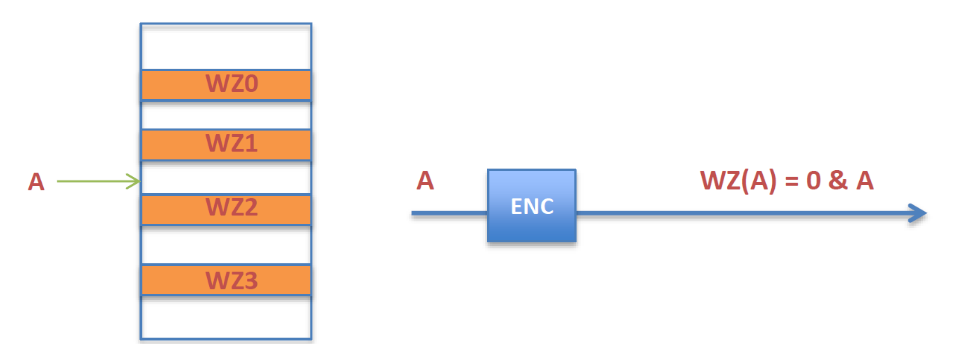
\includegraphics[height=3cm]{images/codifica-fuori-wz.png}
    \caption{ADDR non appartenente a nessuna Working Zone}
    \label{fig:codifica-fuori-wz}
\end{figure}
\item se l'indirizzo da trasmettere (\verb^ADDR^) appartiene ad una Working Zone, il bit addizionale \verb^WZ_BIT^ è posto a 1, mentre i bit di indirizzo vengono divisi in 2 sotto campi rappresentanti:
\begin{itemize}[label=$\circ$]
\item Il numero della working-zone al quale l'indirizzo appartiene \verb^WZ_NUM^, che sarà codificato in binario
\item L'offset rispetto all'indirizzo di base della working zone \verb^WZ_OFFSET^, codificato come one-hot (cioè il valore da rappresentare è equivalente all'unico bit a 1 della codifica).
\end{itemize}
In pratica dato \verb^ADDR^, verrà trasmesso \verb^WZ_BIT=1^ concatenato ad \verb^WZ_NUM^ e \verb^WZ_OFFSET^ (\texttt{WZ\_BIT \& WZ\_NUM \& WZ\_OFFSET}, dove \verb^&^ è il simbolo di concatenazione);
\begin{figure}[H]
    \centering
    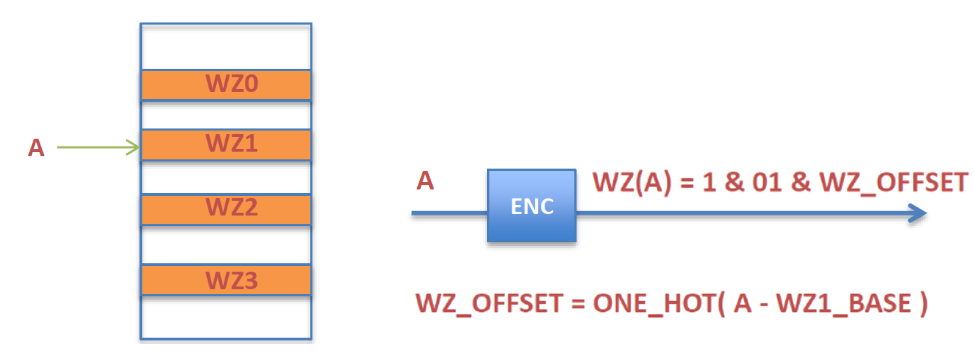
\includegraphics[height=3cm]{images/codifica-dentro-wz.png}
    \caption{ADDR appartenente a una Working Zone}
    \label{fig:codifica-dentro-wz}
\end{figure}
\end{itemize}
Nella versione da implementare il numero di bit da considerare per l'indirizzo da codificare è 7. Il che definisce come indirizzi validi quelli da 0 a 127. Il numero di working-zone è 8 (\verb^Nwz=8^) mentre la dimensione della working-zone è 4 indirizzi incluso quello base (\verb^Dwz=4^). Questo comporta che l'indirizzo codificato sarà composto da 8 bit: 1 bit per \verb^WZ_BIT^ + 7 bit per \verb^ADDR^, oppure 1 bit per \verb^WZ_BIT^, 3 bit per codificare in binario a quale tra le 8 working zone l'indirizzo appartiene, e 4 bit per codificare one hot il valore dell'offset di \verb^ADDR^ rispetto all'indirizzo base.
Il modulo da implementare leggerà l'indirizzo da codificare e gli 8 indirizzi base delle working-zone e dovrà produrre l'indirizzo opportunamente codificato.\pagebreak\\
\underline{Esempio:}\\
La seguente sequenza di numeri mostra un esempio del contenuto della memoria al termine di una elaborazione. I valori che qui sono rappresentati in decimale, sono memorizzati in memoria con l'equivalente codifica binaria su 8 bit senza segno.

\begin{center}
\begin{tabular}{ccccccl}
\hline
\multicolumn{2}{c}{\textbf{Caso 1\textsuperscript{1}}} &  & \multicolumn{2}{c}{\textbf{Caso 2\textsuperscript{2}}} &  & \multicolumn{1}{c}{Commento} \\ \hline
Indirizzo Memoria & Valore &  & Indirizzo Memoria & Valore &  & \multicolumn{1}{c}{} \\
0 & 4 &  & 0 & 4 &  & Indirizzo base WZ 0 \\
1 & 13 &  & 1 & 13 &  & Indirizzo base WZ 1 \\
2 & 22 &  & 2 & 22 &  & Indirizzo base WZ 2 \\
3 & 31 &  & 3 & 31 &  & Indirizzo base WZ 3 \\
4 & 37 &  & 4 & 37 &  & Indirizzo base WZ 4 \\
5 & 45 &  & 5 & 45 &  & Indirizzo base WZ 5 \\
6 & 77 &  & 6 & 77 &  & Indirizzo base WZ 6 \\
7 & 91 &  & 7 & 91 &  & Indirizzo base WZ 7 \\
8 & 42 &  & 8 & 33 &  & ADDR da codificare \\
9 & 42 &  & 9 & 180\textsuperscript{3}&  & Valore codificato in output \\
\multicolumn{1}{l}{} & \multicolumn{1}{l}{} & \multicolumn{1}{l}{} & \multicolumn{1}{l}{} & \multicolumn{1}{l}{} & \multicolumn{1}{l}{} &  \\ \hline
\end{tabular}
\end{center}
\begin{footnotesize}
\textsuperscript{1} con valore non presente in nessuna working zone\\
\textsuperscript{2} con valore presente in una working zone\\
\textsuperscript{3} 1 - 011 - 0100
\end{footnotesize}


\vspace{4mm}
\titlerule[0.4pt]


%%%%%%%%%%%%%%%%%%%%%%%%%%%%%%%%%%%%%%%%%%%%
%%%%%%%%%%%%%%% ARCHITETTURA %%%%%%%%%%%%%%%
%%%%%%%%%%%%%%%%%%%%%%%%%%%%%%%%%%%%%%%%%%%%
\pagebreak
\section{Architettura}
La specifica progettuale si traduce nel realizzare un'implementazione in grado di leggere i valori contenuti nelle working zone e l'indirizzo da codificare, quindi verificare se quest'ultimo è presente o meno in una WZ ed effettuare di conseguenza l'opportuna codifica.

\subsection{Macchina a Stati Finiti} \label{FSM-section}
Il funzionamento alla base del componente è stato implementato attraverso una FSM che evolve di stato in stato in modo sequenziale ad ogni ciclo di clock (\verb^-^) oppure al variare dei segnali di ingresso \verb^i_start^ e \verb^i_rst^.\\Ciò che ogni stato rappresenta è spiegato più nel dettaglio in tabella \ref{tab:FSM}.

\begin{figure}[H]
    \centering
    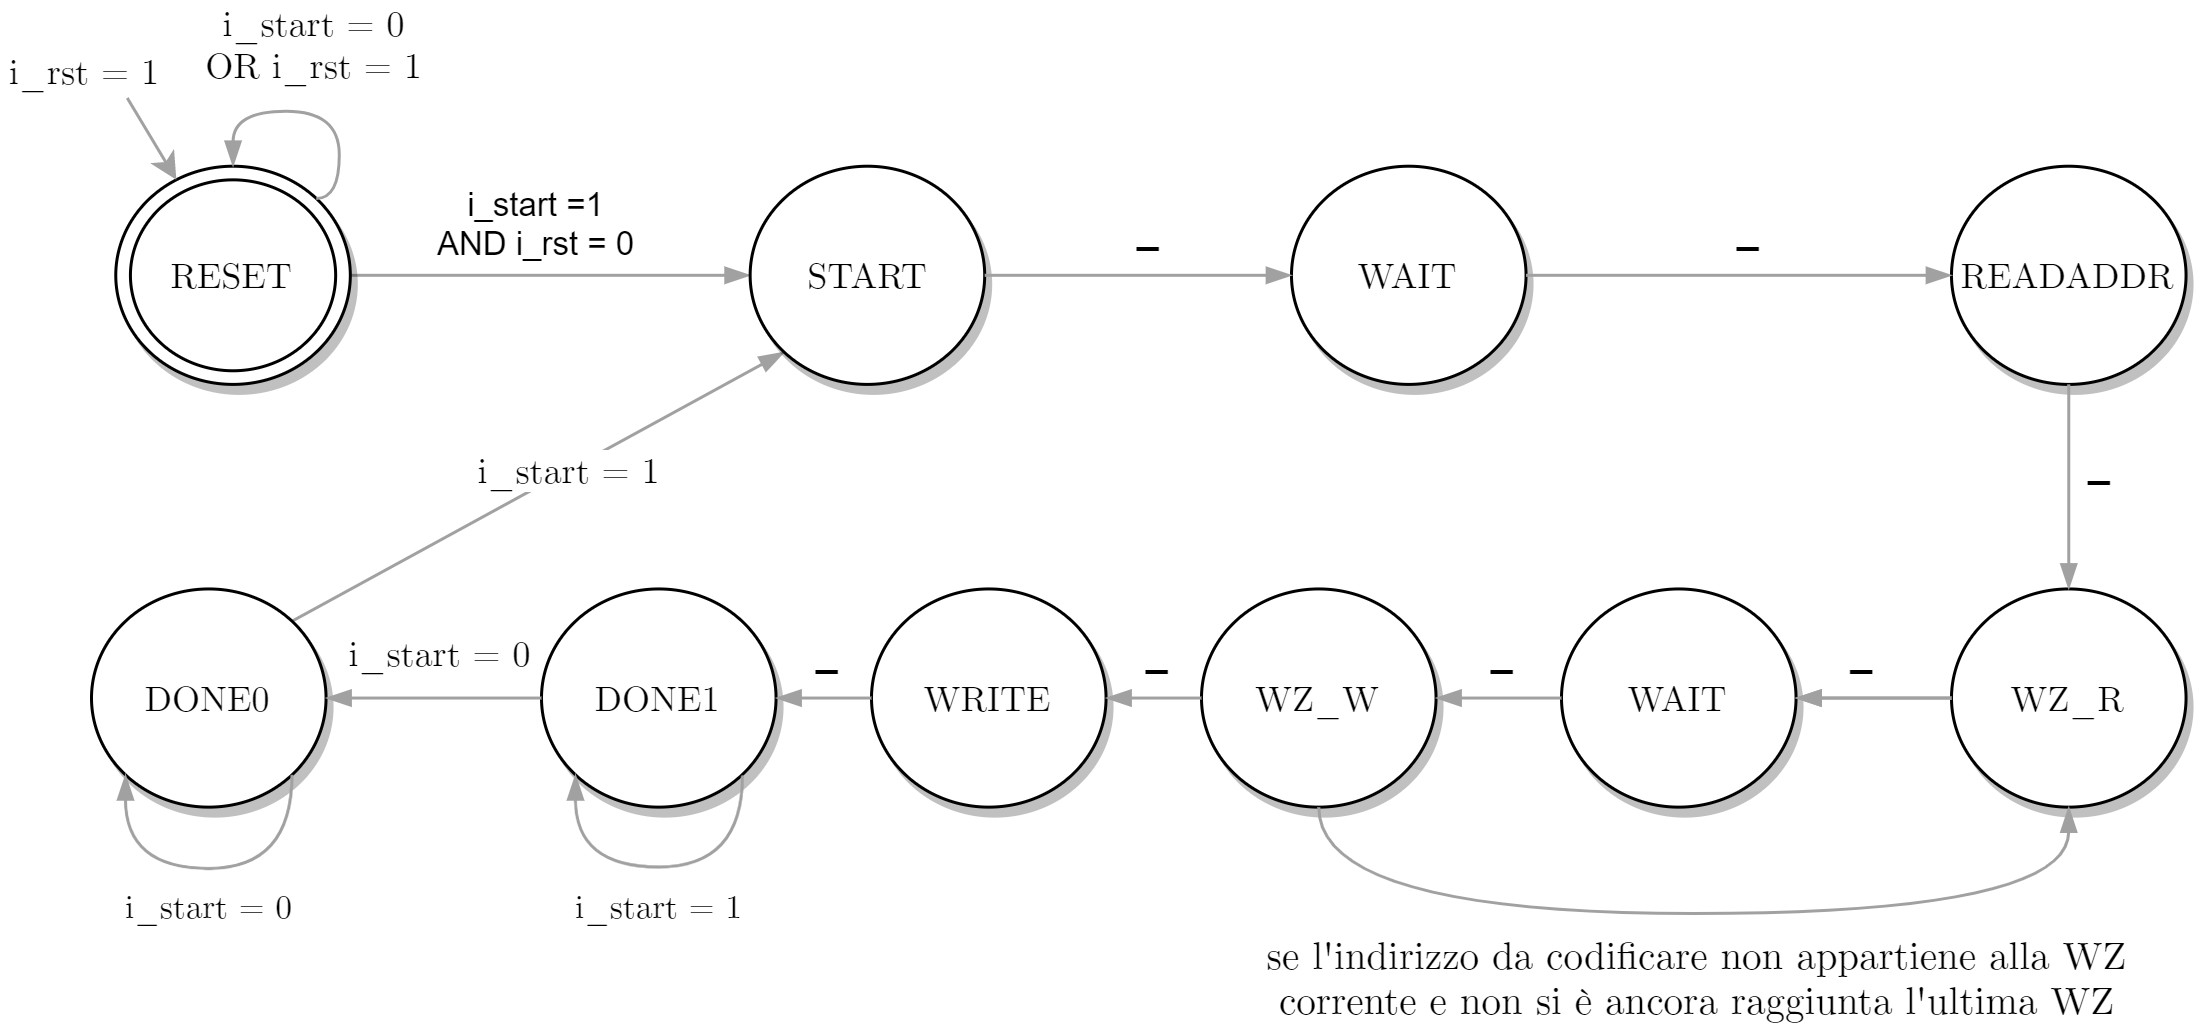
\includegraphics[width=1.0\textwidth]{images/FSM.png}
    \caption{Macchina a Stati Finiti implementata}
    \label{fig:FSM}
\end{figure}



\setlength\intextsep{0mm}
\begin{table}[H]
    \centering
    \caption{Stati della FSM}
    {\tabulinesep=1mm
    \begin{tabu*} to 1.0\textwidth { | X[1c] | X[4.0m] | }
        \hline
        \verb^RESET^ & Stato di partenza della FSM e stato in cui si andrà in presenza di un segnale \verb^i_rst^ (sincrono o asincrono). Alla ricezione di un segnale \verb^i_start^ si passa allo stato \verb^START^. \\
        \hline
        \verb^START^ & Stato iniziale. In questo stato viene richiesta la lettura dalla RAM dell'indirizzo da codificare. \\
        \hline
        \verb^WAIT^ & Stato di attesa per garantire alla memoria il tempo di inviare il dato richiesto. \\
        \hline
        \verb^READADDR^ & Stato in cui il componente legge (riceve) e salva in un registro l'indirizzo da codificare (ADDR). \\
        \hline
        \verb^WZ_R^ & Stato nel quale viene richiesta la lettura dalla RAM dell'indirizzo contenuto nella WZ corrente. \\
        \hline
        \verb^WZ_W^ & Stato nel quale avviene il confronto tra valore da codificare (ADDR) e valore contenuto nella WZ corrente. Se:
        \begin{itemize}
        \setlength\itemsep{0em}
        \item ADDR appartiene alla WZ, effettua la codifica e passa allo stato \verb^WRITE^
        \item ADDR non appartiene alla WZ e si è raggiunta l'ultima WZ, effettua la codifica per indirizzi non appartenenti ad una WZ
        \item ADDR non appartiene alla WZ, passa alla WZ successiva
        \end{itemize}
        \\
        \hline
        \verb^WRITE^ & Stato nel quale viene scritto in output il valore codificato. \\
        \hline
        \verb^DONE1^ & Stato in cui si segnala che il risultato è stato scritto in RAM: \verb^o_done^ è portato ad '1'. Alla ricezione di \verb^i_start^ uguale a '0' si porta la macchina in \verb^DONE0^ per una possibile successiva elaborazione. \\
        \hline
        \verb^DONE1^ & Stato nel quale si rimane in attesa di una possibile successiva elaborazione: \verb^o_done^ è portato a '0'. Alla ricezione di \verb^i_start^ uguale a '1' si riporta la macchina in \verb^START^. \\
        \hline
    \end{tabu*}}
    \label{tab:FSM}
\end{table}

\subsection{Implementazione}
A livello implementativo si è optato per una FSM \textit{single-process}, in modo da realizzare un algoritmo di semplice stesura, interpretazione e manutenzione, evitando così anche eventuali problemi di sincronizzazione tra più processi.

\subsubsection{Interfaccia}
L'interfaccia del componente è stata presentata nelle specifiche nel seguente modo:
\begin{figure}[H]
    \centering
    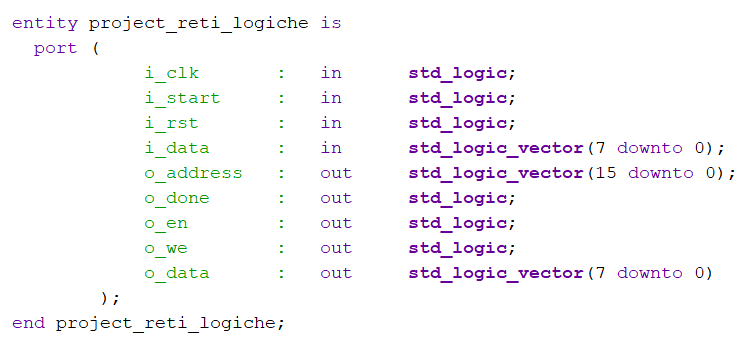
\includegraphics[height=6cm]{images/interfaccia.png}
    \caption{Interfaccia}
    \label{fig:interfaccia}
\end{figure}
\noindent\\
Tale componente si interfaccia, inoltre, con un chip RAM in cui sono caricati tutti i dati
necessari all'elaborazione.

\subsubsection{Segnali}
Sono stati definiti i seguenti segnali:
\begin{figure}[H]
    \centering
    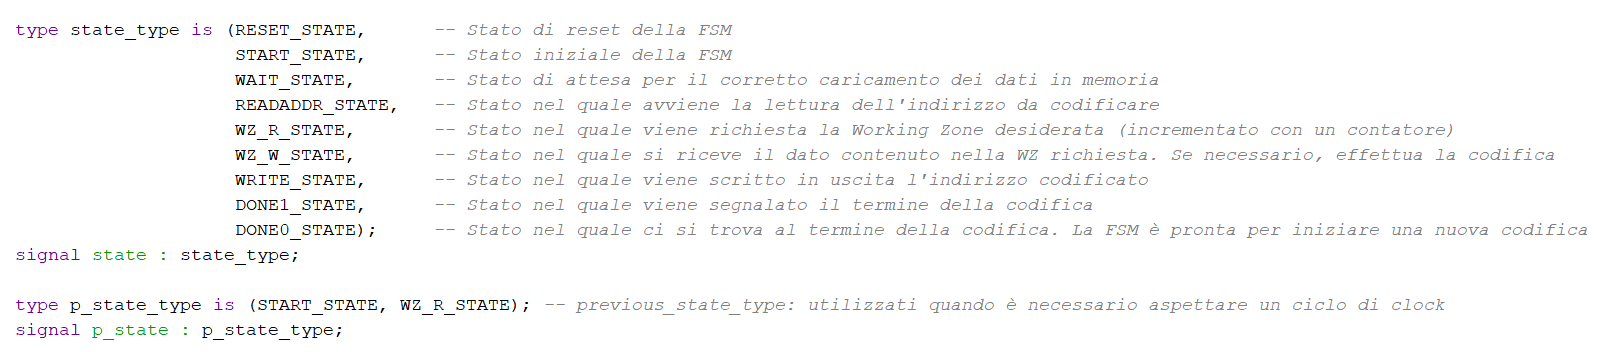
\includegraphics[width=1.0\textwidth]{images/segnali.png}
    \caption{Segnali}
    \label{fig:segnali}
\end{figure}
\noindent\\
I segnali definiti sono quindi utilizzati per la definizione degli stati della macchina a stati.

\subsubsection{Variabili}
Poiché la FSM realizzata è mono-processo, si è fatto un discreto utilizzo delle variabili:
\begin{figure}[H]
    \centering
    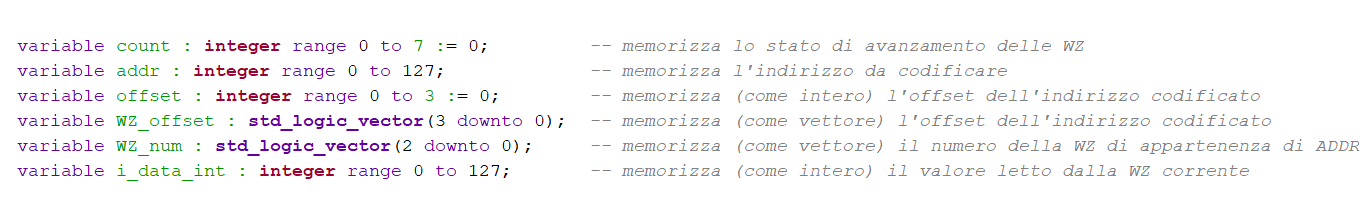
\includegraphics[width=1.0\textwidth]{images/variabili.png}
    \caption{Variabili}
    \label{fig:variabili}
\end{figure}

\pagebreak
\subsubsection{Algoritmo}
Gli stati della FSM e il loro avanzamento sequenziale sono già stati descritti nella sezione "\nameref{FSM-section}" a pagina \pageref{FSM-section}.\\\\
Vediamo ora un riassunto dell'algoritmo di esecuzione:
\begin{enumerate}
\item Si accende la macchina e ci si pone subito nello stato di RESET, nel quale si rimane finché non viene ricevuto un segnale di start
\item Nello stato di START viene attivata la comunicazione con la memoria e viene richiesto il dato contenuto in RAM(8), ovvero l'indirizzo ADDR da codificare
\item Viene ricevuto e salvato in una variabile il dato richiesto (ADDR)
\item Per ogni working zone:
\begin{enumerate}
\item viene richiesto il dato contenuto nella working zone corrente
\item viene ricevuto il dato richiesto
\item viene confrontato tale dato con ADDR per capire se quest'ultimo appartiene o meno a tale WZ
\item se appartiene, viene codificato come da specifica. Altrimenti si passa alla WZ successiva.\\
In caso si sia raggiunta l'ultima WZ, ADDR viene codificato come indirizzo fuori working-zone
\end{enumerate}
\item Quando ADDR viene codificato, si interrompe il ciclo di lettura delle WZ (se non si è ancora raggiunta l'ultima) e si procede a scrivere in output su RAM(9) il valore codificato
\item Viene quindi segnalato che il dato è stato scritto e che è possibile iniziare una eventuale nuova codifica
\end{enumerate}
\noindent\\
N.B: in caso di ricezione del segnale di reset, si ritorna immediatamente nello stato RESET interrompendo l'elaborazione corrente.\\\\
Vediamo ora nel dettaglio cosa accade quando viene effettuato il confronto tra ADDR e la WZ corrente (ciò avviene nello stato \verb^WZ_W_STATE^):\\\\
\begin{figure}[H]
    \centering
    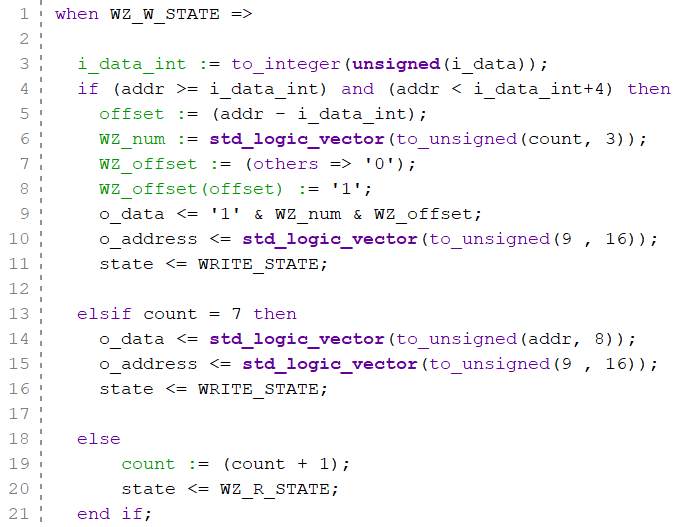
\includegraphics[height=10cm]{images/wz-w-state.png}
    \caption{WZ\_W\_STATE}
    \label{fig:wz-w-state}
\end{figure}
\newpage

\begin{itemize}[align=left, labelwidth=4em, leftmargin=1.8cm]
\item[Linea 3.] Lettura, conversione ad intero e salvataggio del valore contenuto nella WZ corrente
\item[Linea 4.] Viene controllato se ADDR appartiene alla WZ corrente, sfruttando il fatto che, da specifica, la dimensione di una Working Zone è 4 indirizzi \verb^(Dwz=4)^. Se appartiene...
\begin{itemize}[align=left, labelwidth=4em, leftmargin=1.8cm]
\item[Linea 5.] Viene calcolato l'offset (intero) come sottrazione tra il valore di ADDR l'indirizzo base della WZ
\item[Linea 6.] Viene convertito il numero della WZ da intero a vettore logico di 3 bit, utilizzando la variabile \verb^count^ che tiene memorizzato il numero della WZ corrente
\item[Linea 7.] Viene inizializzato a 0 il vettore logico dell'offset
\item[Linea 8.] Il bit in posizione \verb^offset^-esima viene posto a 1. Questo realizza la codifica one-hot dell'offset 
\item[Linea 9.] Viene costruito l'indirizzo codificato, come concatenazione dei vettori logici riportati (come da specifica)
\item[Linea 10.] Viene indicato su quale indirizzo della RAM andare a scrivere il valore codificato
\item[Linea 11.] Ci si sposta nello stato \verb^WRITE_STATE^
\end{itemize}
\item[Linea 13.] Se si è raggiunta l'ultima WZ e non si è ancora trovato un riscontro con le WZ...
\begin{itemize}[align=left, labelwidth=4em, leftmargin=1.8cm]
\item[Linea 14.] Viene posto in output ADDR così com'è stato letto, senza alcuna codifica ulteriore
\item[Linea 15.] Viene indicato su quale indirizzo della RAM andare a scrivere il valore in output
\item[Linea 16.] Ci si sposta nello stato \verb^WRITE_STATE^
\end{itemize}
\item[Linea 18.] Se non si è trovato un riscontro con la WZ corrente e non si è ancora raggiunta l'ultima WZ...
\begin{itemize}[align=left, labelwidth=4em, leftmargin=1.8cm]
\item[Linea 19.] Si incrementa di uno il valore della variabile \verb^count^
\item[Linea 20.] Si passa allo stato \verb^WZ_R_STATE^, nel quale si andrà a richiedere la lettura della WZ successiva, per poi ritornare nuovamente in questo stato (\verb^WZ_W_STATE^)
\end{itemize}

\end{itemize}


\vspace{4mm}
\titlerule[0.4pt]


%%%%%%%%%%%%%%%%%%%%%%%%%%%%%%%%%%%%%%%
%%%%%%%%%%%%%%% SINTESI %%%%%%%%%%%%%%%
%%%%%%%%%%%%%%%%%%%%%%%%%%%%%%%%%%%%%%%
\pagebreak
\section{Sintesi}
\subsection{Report di sintesi}
Analizzando il "Vivado Synthesis Report" troviamo che la FSM è stata codificata in one-hot, per migliorarne l'efficienza:

\begin{verbatim}
---------------------------------------------------------------------------------------------------
                   State |                     New Encoding |                Previous Encoding 
---------------------------------------------------------------------------------------------------
             reset_state |                        000000001 |                             0000
             start_state |                        000000010 |                             0001
              wait_state |                        000000100 |                             0010
          readaddr_state |                        000001000 |                             0011
              wz_w_state |                        000010000 |                             0101
             write_state |                        000100000 |                             0110
             done1_state |                        001000000 |                             0111
             done0_state |                        010000000 |                             1000
              wz_r_state |                        100000000 |                             0100
---------------------------------------------------------------------------------------------------
\end{verbatim}
\noindent
Dal report di sintesi possono essere inoltre estratte le seguenti informazioni riguardo i registri e i mux:

\begin{center}
\begin{minipage}{14cm}
\begin{small}
\begin{verbatim}
+---Adders :                                    +---Registers : 
	   3 Input      9 Bit       Adders := 1	   	       16 Bit    Registers := 1  
	   2 Input      3 Bit       Adders := 1	   	       8 Bit    Registers := 1  
	   3 Input      2 Bit       Adders := 1	   	       7 Bit    Registers := 1
                                           	   	   3 Bit    Registers := 1
                                           	   	   1 Bit    Registers := 4
\end{verbatim}
\end{small}
\end{minipage}
\end{center}
\begin{center}
\begin{minipage}{8cm}
\begin{small}
\begin{verbatim}
+---Muxes : 
	   9 Input     16 Bit        Muxes := 1     
	   9 Input      9 Bit        Muxes := 1     
	   2 Input      9 Bit        Muxes := 6     
	   2 Input      8 Bit        Muxes := 1     
	   9 Input      3 Bit        Muxes := 1     
	   2 Input      1 Bit        Muxes := 1     
	   3 Input      1 Bit        Muxes := 1     
	   9 Input      1 Bit        Muxes := 8
\end{verbatim}
\end{small}
\end{minipage}
\end{center}

\subsection{Area occupata}
Eseguendo un "Report Utilization" vediamo ora l'area occupata dal design sintetizzato.\\E' da notare che si è voluta ottimizzare l'area occupata dal componente, non tanto per limiti di disponibilità della FPGA utilizzata\footnote{xc7a200tfbg484-1} (che come possiamo vedere, i valori di utilizzo hanno svariati ordini di grandezza in meno rispetto alla disponibilità della FPGA), ma in previsione di poter utilizzare tale algoritmo su FPGA molto più piccole.\\
\begin{table}[H]
    \centering
   
    \begin{tabu*} to 1.0\textwidth { | X[1.0] | X[1.0] | X[1.0] | X[1.0] | }
        \hline
        \textbf{Risorsa} & \textbf{Utilizzo} & \textbf{Disponibilità} & \textbf{Utilizzo in \%} \\
         \hline
         Look Up Table & 41 & 134600 & 0.03\% \\
         \hline
         Flip Flop & 35 & 269200 & 0.01\% \\
         \hline
    \end{tabu*}
    \caption{Report di utlizzo}
    \label{tab:utilization-report}
\end{table}

\subsection{Report di timing}
Analizzando il report di timing si può vedere quanto è veloce in un singolo ciclo di clock il design sintetizzato. Si è ottenuto con il clock della specifica di 100ns un Worst Negative Slack pari a 95,354ns. Da questo valore, sapendo anche il ritardo di riposta della RAM (T\textsubscript{RAM}), possiamo calcolare il periodo minimo applicabile al design creato:
\begin{align*}
    &T_{min} = T_{curr} - \mathit{WNS} + T_{RAM} = 100ns - 95.354ns + 1ns = 5.646ns
\end{align*}
Il design creato ha quindi una massima frequenza di clock pari a: \( f_{max} = 1/T_{min} \approx 177.1 \mathit{Mhz} \).\\

\vspace{4mm}
\titlerule[0.4pt]


%%%%%%%%%%%%%%%%%%%%%%%%%%%%%%%%%%%%%%%%%%%
%%%%%%%%%%%%%%% SIMULAZIONI %%%%%%%%%%%%%%%
%%%%%%%%%%%%%%%%%%%%%%%%%%%%%%%%%%%%%%%%%%%
\pagebreak
\section{Simulazioni}
Per verificare il corretto funzionamento del design, sono stati creati dei test bench appositi al fine di testare il componente sia nei normali casi di utilizzo sia nei casi limite. Di seguito sono riportati i test bench più significativi.

\subsection{Test Bench 0 (forniti con la specifica)}
In questi test bench viene verificato il corretto funzionamento nei due casi base, ovvero l'appartenenza o meno dell'indirizzo da codificare all'interno di una working-zone.

\subsubsection{Behavioral Simulation}
In questo primo test, l'indirizzo da codificare è presente nella Working Zone 3. Come possiamo vedere dalla waveform, per prima cosa viene letto l'indirizzo da codificare e successivamente si passa alla lettura delle WZ. Arrivati alla terza WZ, viene individuato un riscontro e pertanto viene effettuata la codifica e la scrittura, quindi viene segnalato il termine dell'elaborazione.\\
\begin{figure}[H]
    \centering
    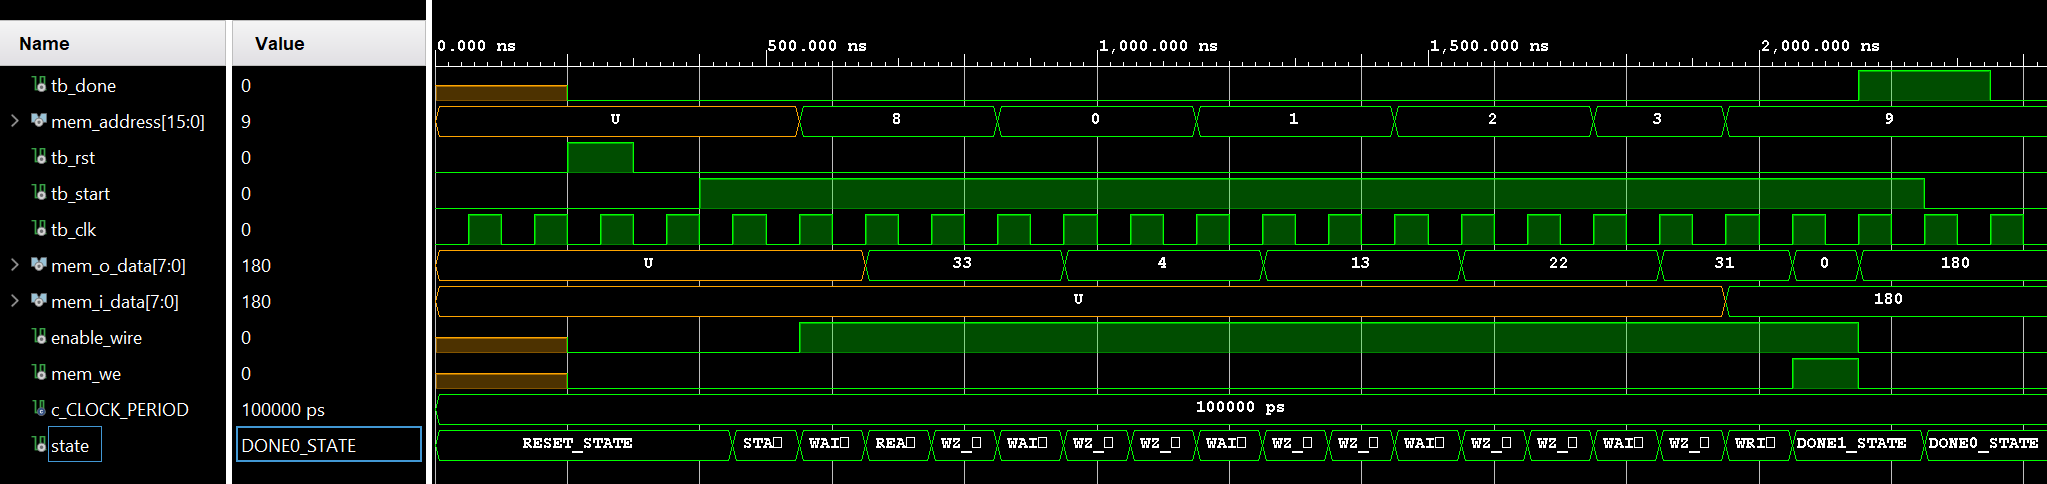
\includegraphics[width=1.0\textwidth]{images/test-in-wz.png}
    \caption{L'indirizzo da codificare è presente nella Working Zone 3}
    \label{fig:test-in-wz}
\end{figure}
\noindent\\ Nel secondo test, l'indirizzo da codificare (ADDR) non è presente in alcuna Working Zone. Pertanto, vengono lette tutte le WZ e quindi ADDR viene scritto in output così com'è stato letto (come da specifica).\\
\begin{figure}[H]
    \centering
    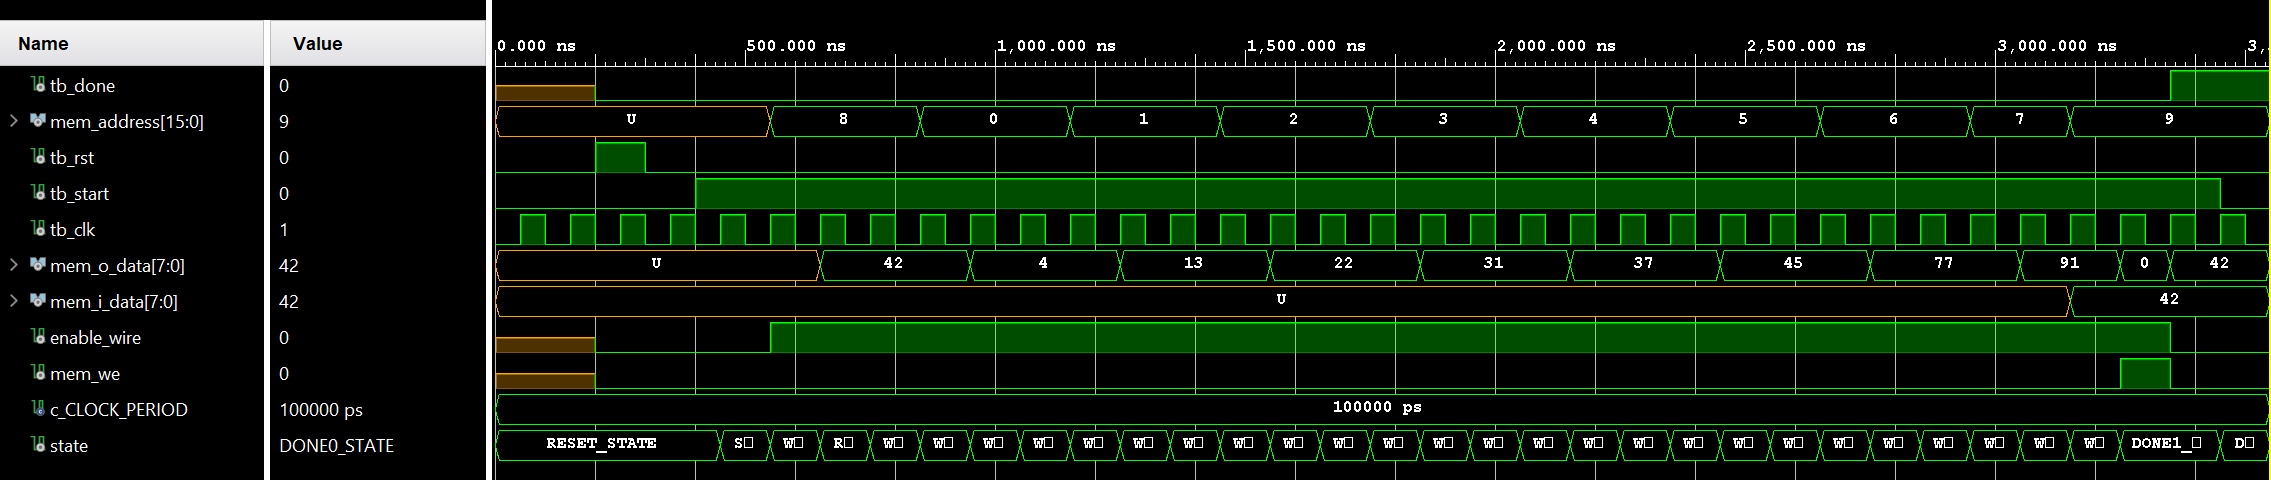
\includegraphics[width=1.0\textwidth]{images/test-no-wz.png}
    \caption{L'indirizzo da codificare non è presenta in alcuna Working Zone}
    \label{fig:test-no-wz}
\end{figure}

\subsubsection{Post-Synthesis Functional Simulation}
\noindent Come possiamo vedere, ripetendo in post-sintesi il test bench rappresentato dalla Figura \ref{fig:test-in-wz}, i valori che prima risultavano non inizializzati ("U") ora spariscono e vengono rimpiazzati da valori reali, questi valori sono ininfluenti e sono dati dalle ottimizzazioni fatte dal tool di sintesi.\\
\begin{figure}[H]
    \centering
    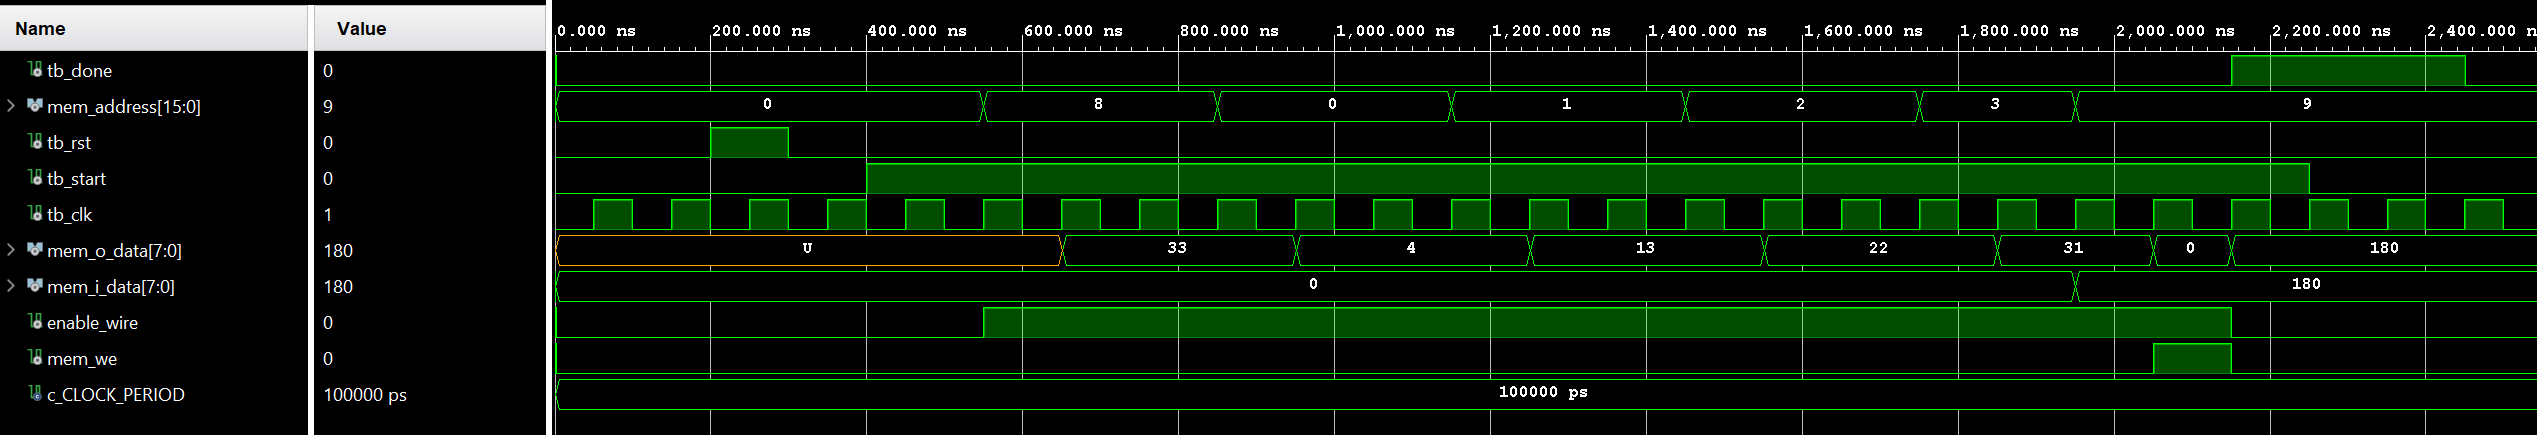
\includegraphics[width=1.0\textwidth]{images/test-in-wz-post.png}
        \caption{Waveform dei segnali in Post-Synthesis Timing Simulation. Test bench della Figura \ref{fig:test-in-wz}}
    \label{fig:test-in-wz-post}
\end{figure}

\subsection{Test Bench 1: Multi Start}
Si è poi effettuato un test per verificare il corretto funzionamento nel caso di conversioni in sequenza, senza reset delle Working Zone.\\
\begin{figure}[H]
    \centering
    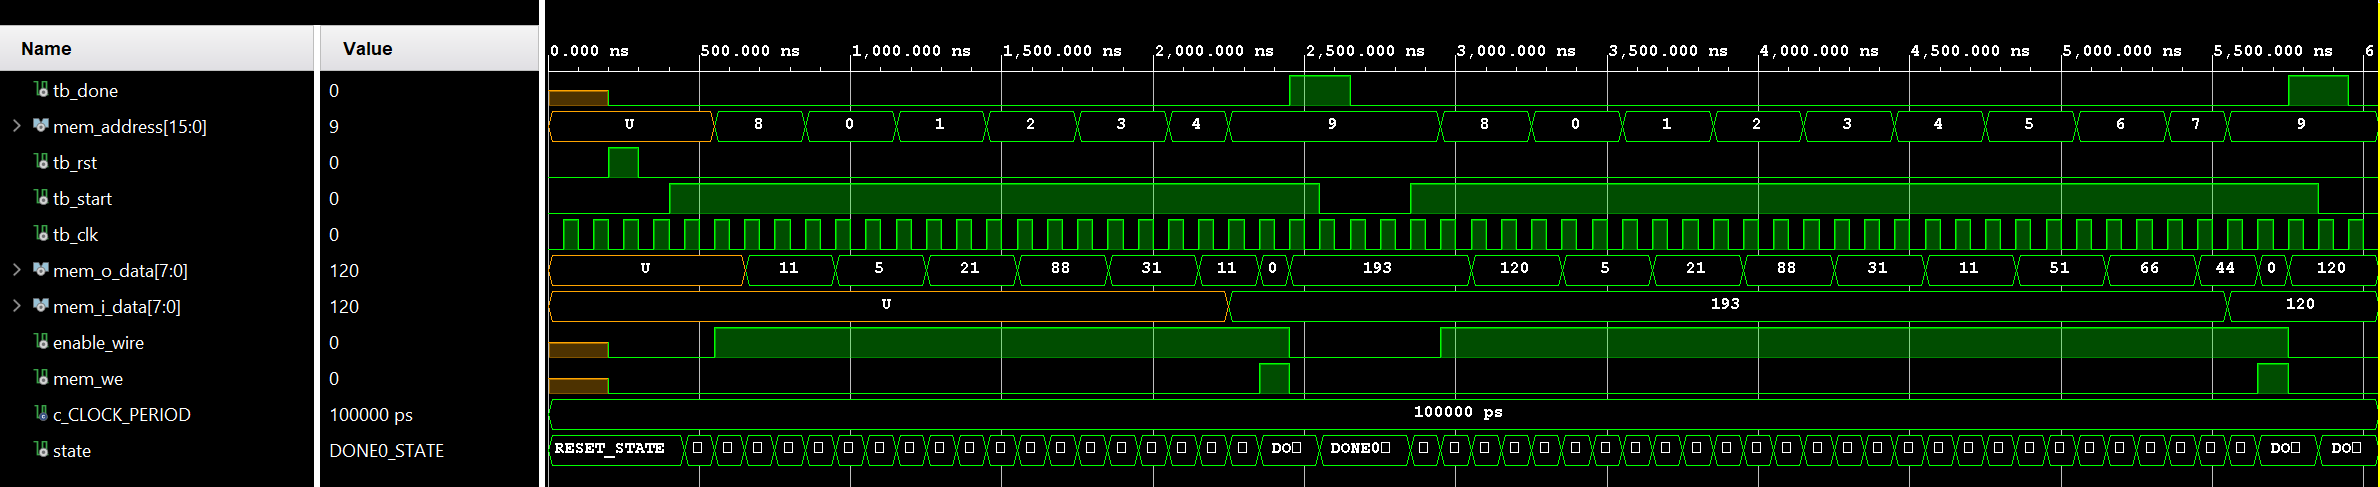
\includegraphics[width=1.0\textwidth]{images/test-multi-start.png}
        \caption{Segnali di start multipli}
    \label{fig:test-multi-start}
\end{figure}
\noindent\\ In questo caso, nel primo start viene trovato un riscontro tra ADDR e la WZ numero 3, mentre nel secondo start non viene trovato alcun riscontro.

\subsection{Test Bench 2: Multi Reset}
Un ulteriore test effettuato è quello nel caso in cui si verifichi un reset al termine della prima elaborazione, prima del secondo start. Da specifica, solo tramite reset si può verificare un cambiamento delle WZ. Questo test verifica la corretta lettura delle nuove Working Zone.\\
\begin{figure}[H]
    \centering
    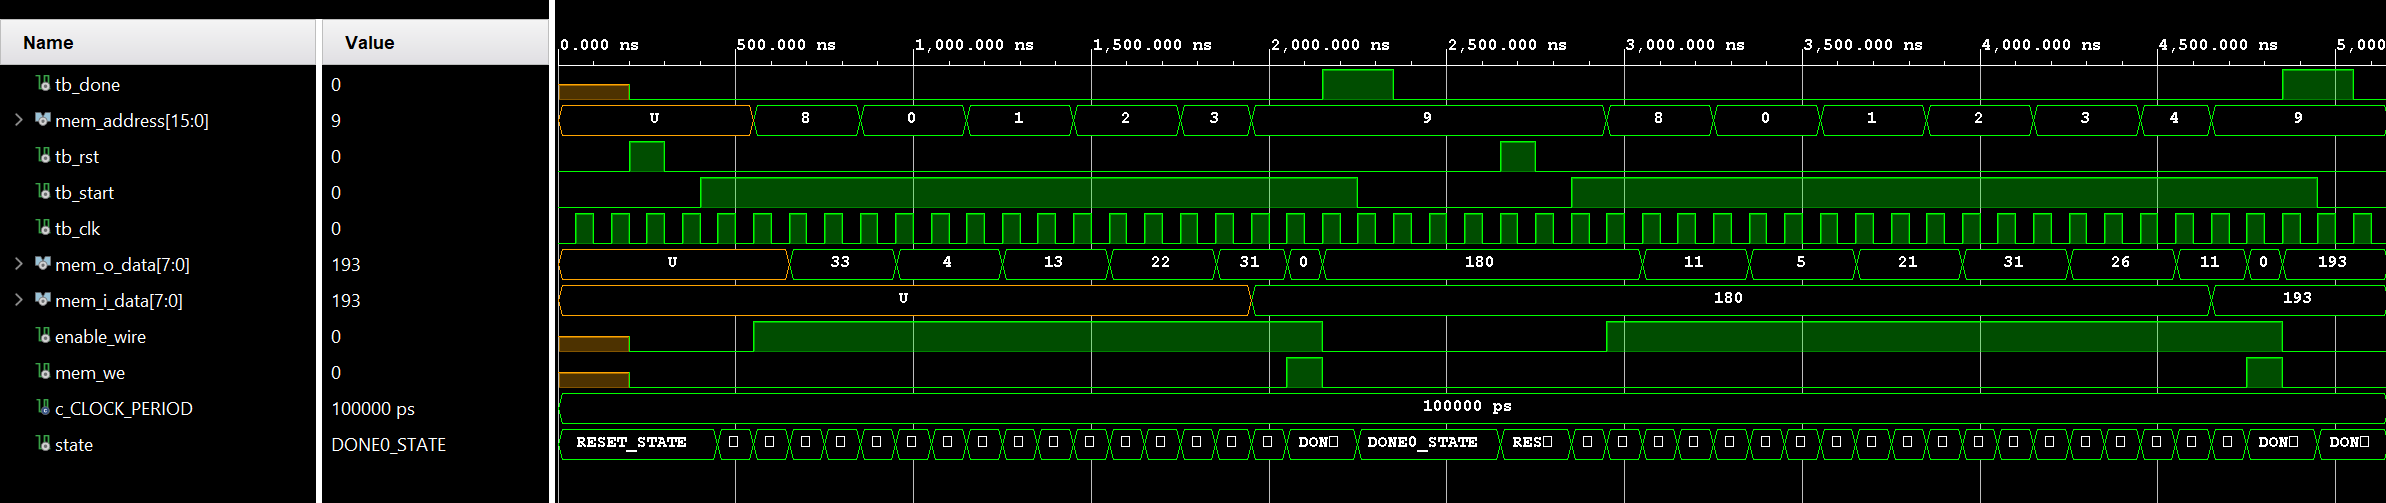
\includegraphics[width=1.0\textwidth]{images/test-multi-reset.png}
        \caption{Segnali di reset multipli}
    \label{fig:test-multi-reset}
\end{figure}
\noindent\\ In questo caso, in entrambi gli start viene trovato un riscontro tra ADDR e una WZ, ma prima del secondo start è stato effettuato un reset, con conseguente cambio delle WZ.

\subsection{Test Bench 3: Reset Asincrono}
Un particolare caso limite è quello che si genera quando viene ricevuto un segnale di reset in modo asincrono durante una elaborazione in corso, iniziata a seguito di uno start.\\Come possiamo vedere dal test, il componente ha inizialmente avviato la normale elaborazione, leggendo prima ADDR e poi ciclando sulle varie WZ. Alla ricezione del segnale di reset, il componente è ritornato nello stato di \verb^RESET^ per poi iniziare da capo l'elaborazione, in quanto il segnale di start è nuovamente alto.\\ 
\begin{figure}[H]
    \centering
    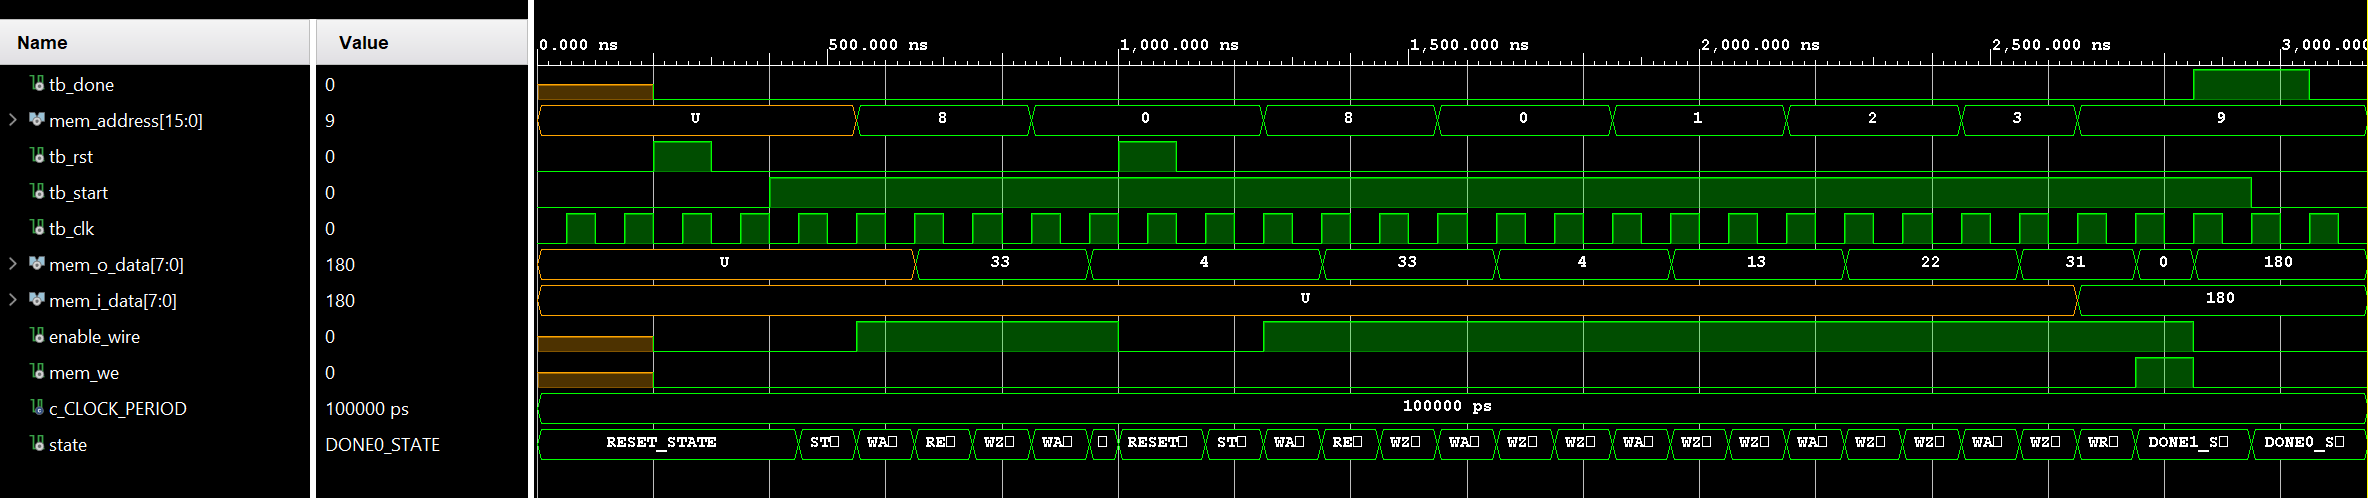
\includegraphics[width=1.0\textwidth]{images/test-reset-async.png}
        \caption{Segnali di reset asincrono}
    \label{fig:test-reset-async}
\end{figure}

\pagebreak
\subsection{Altri test}
Sono inoltre stati effettuati i seguenti test:
\begin{itemize}
\item Working Zone adiacenti, per verificare che il componente riconosca la WZ corretta
\item Reset Asincroni multipli, di breve durata, per verificare il corretto comportamento anche in condizioni di stress
\item Unione di tutti i test precedenti con centinaia di elaborazioni (WZ generate in modo randomico), per verificare contemporaneamente tutte le casistiche durante un'elaborazione prolungata
\end{itemize}

\vspace{4mm}
\titlerule[0.4pt]


%%%%%%%%%%%%%%%%%%%%%%%%%%%%%%%%%%%%%%%%%%%
%%%%%%%%%%%%%%% CONCLUSIONE %%%%%%%%%%%%%%%
%%%%%%%%%%%%%%%%%%%%%%%%%%%%%%%%%%%%%%%%%%%
\section{Conclusione}
Riassumendo, si è creato un design con le seguenti caratteristiche:
\begin{itemize}
    \item Funzionante in pre e post-sintesi (Functional e Timing).
    \item Ottimizzato in modo da ridurre il più possibile l'area occupata.
    \item Frequenza massima di clock impostabile a 177.1Mhz.
    \item Utilizzo di LUT pari al 0.03\%.
    \item Utilizzo di FF pari al 0.01\%
\end{itemize}

\subsection{Nota aggiuntiva sull'ottimizzazione}
Come già indicato più volte, si è deciso di seguire la scelta progettuale di ottimizzare l'area occupata dai componenti di memoria, nell'ottica di rendere possibile l'utilizzo di tale componente su FPGA di dimensioni ben più ridotte di quella utilizzata in fase di progettazione.\\\\Si è però consapevoli che un'altra ottimizzazione possibile fosse quella di migliorare il componente dal punto di vista delle prestazioni, a discapito dell'area occupata. Infatti, il componente realizzato non mantiene salvate in memoria le Working Zone lette durante l'elaborazione, ma le rilegge ad ogni nuovo start.
Poiché da specifica le WZ possono cambiare solo a seguito di un reset, sarebbe stato possibile salvarle alla prima elaborazione e quindi riutilizzarle ad ogni nuova elaborazione, dovendo così leggere dalla RAM solamente l'indirizzo ADDR da codificare. In caso di reset, queste sarebbero state rilette e salvate nuovamente.\\A scopo didattico, si è provato a realizzare anche questa seconda implementazione, ottenendo un componente di area quadrupla rispetto alla prima implementazione, con un leggero miglioramento di prestazioni in caso di migliaia di elaborazioni senza reset.

\end{document}
